% Compact single-column motivation, introduced at its first reference.
\begin{figure}[t]
  \centering
  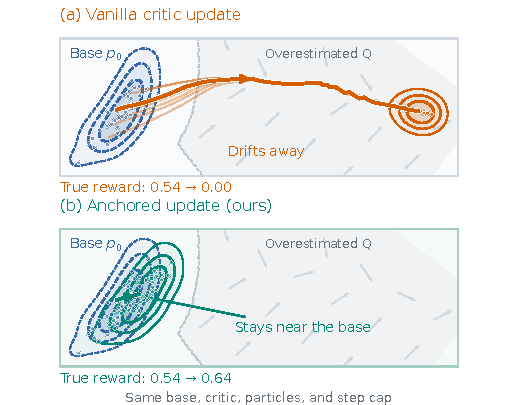
\includegraphics[width=\linewidth]{figures/problem_motivation.pdf}
  \caption{\textbf{Preserving pretrained robot skills during refinement.}
  In robot manipulation, refinement should correct placement or release
  errors while preserving useful reaching and grasping behavior. This
  synthetic action-space example illustrates how critic-guided updates
  can disrupt pretrained actions. Both panels share a frozen critic,
  paired initial actions from the blue base distribution, and a per-update
  step cap. (a) Critic ascent moves actions
  into an overestimated region (gray), reducing true reward. (b) Projection
  around each initial action preserves a fixed base reference and improves
  reward. Curves show representative updates; contours enclose $50\%$,
  $80\%$, and $95\%$ of estimated action probability.}
  \label{fig:problem}
\end{figure}
